\documentclass[12pt]{article}
\usepackage[margin = 0.9in, top=0.8in]{geometry}
\usepackage{graphicx}
\usepackage{textgreek}
\usepackage{amsmath}
\usepackage{amsfonts}
\usepackage{mathtools}
\usepackage{amssymb}
\usepackage{float}
\usepackage{subcaption}
%\usepackage{algorithm}
%\usepackage{algorithmic}
%\usepackage[noend]{algpseudocode}
\usepackage[english]{babel}
\newtheorem{theorem}{Theorem}
\usepackage[ruled, lined, linesnumbered, commentsnumbered, longend]{algorithm2e}
\usepackage{hyperref}
\usepackage{grffile}
\graphicspath{{./2/images},{./2/data}, {./}}
\usepackage{hyperref}
\usepackage{grffile}
\graphicspath{{./2/images},{./}}
\title{CS 754 - Advanced Image Processing\\Assignment 4 - Report}
\author{Shaan ul Haque - 180070053\\Mantri Krishna Sri Ipsit - 180070032}
\newcommand{\norm}[1]{\left\lVert #1 \right\rVert}
\newcommand{\R}{\mathbb{R}}
\newcommand{\A}{\mathcal{A}}
\SetKwInOut{KwA}{Assumption}
\SetKwInOut{KwIn}{Input}
\SetKwInOut{KwOut}{Output}
\SetKwInOut{KwInit}{Initialization}
\SetKwInOut{KwIter}{Iteration}
\SetKwInOut{KwRep}{repeat}
\SetKwInOut{KwDef}{Define}
\begin{document}
	
	\maketitle
\section*{Question 1}
\subsection*{1.a}
The equation (7) given in the paper is as follows:
$$J_3(v) = \sum \limits_j \rho_j (A_{j\rightarrow}v - b_j)$$
Here $A_{j\rightarrow}$ represents a matrix of derivative filters centered on pixel $j$ to be applied on vectorized image $I_1$ i.e, $v$. If the pixel $j \in S_1$, then as per equation (6), we have to subtract the gradient of original image $I$ and then apply $\rho$. Hence when $j \in S_1$, $b_j$  has the derivative of $I$ centered at $j$. \newline
When $j \in S_2$, as per equation (6), we apply $\rho$ directly on the derivative of $I_1$ centered at $j$. Hence in this case the value of $b_j=0$ when $j \in S_2$.
\subsection*{1.b}
\begin{itemize}
	\item The following terms are obtained from the likelihood:
	$$\rho(f_{i,k}\cdot I_1) + \rho(f_{i,k}\cdot (I-I_1))$$
	\item The following terms are obtained from the prior:
	$$f_{i,k} \cdot I_1, f_{i,k}\cdot (I-i_1)$$ 
\end{itemize}
The log-histogram of derivative filters was the prior used in the paper. The Laplacian mixture model was used as the likelihood in the paper.
\subsection*{1.c}
The paper exploits the statistics of natural images. It is known that the log-histograms of the derivative filters have a sparse distribution. They lie below the straight line connecting the minimal and maximal values. The Gaussian distribution is not sparse because it is always above the straight line. The Laplacian distribution is exactly at the border between sparse and non-sparse distributions. This prior has been used because the sparse nature of derivative filter outputs is a robust property of natural images and this paper focuses on removing reflections from natural images.
\begin{figure}[ht]
	\centering
	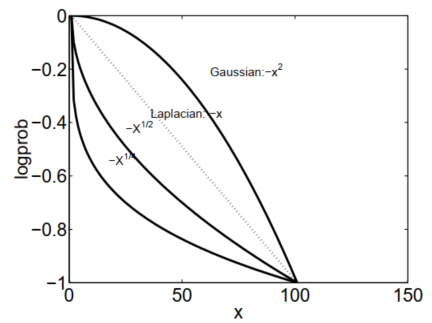
\includegraphics[scale=1]{log_histograms.png}
	\caption{Sparness of different distributions (taken from the paper provided). The Laplacian distribution is exactly at the border between sparse and non-sparse. Any distribution lying above Laplacian is non-sparse and any distribution lying below Laplacian is sparse.}
\end{figure}
\section*{Question 2}
Given model:
\begin{equation*}
	\boldsymbol{y} = \boldsymbol{\Phi x} + \boldsymbol{\eta}
\end{equation*}
where $\eta ~ \textit{N}(0, \sigma^2\boldsymbol{I}_{m\times m})$, $\boldsymbol{\Phi} ~ \textit{N}(0, 1/m)$, $\sigma = 0.01\times$ the average absolute value of in $\boldsymbol{\Phi x}$ and $\boldsymbol{x}$ is also drawn from a Gaussian distribution whose mean is zero while the covariance matrix($\boldsymbol{\Sigma_x}$) has polynomial decrement in eigenvalues.\\
The MAP for estimating $\boldsymbol{x}$ given $\boldsymbol{y}, \boldsymbol{\Phi}$ and $\boldsymbol{\Sigma_x}$ is:
\begin{equation*}
	\boldsymbol{x} = argmax_{\boldsymbol{x}} p(x|y)
\end{equation*}
Using Bayes rule, we get:
\begin{equation*}
	argmax_{\boldsymbol{x}} p(x|y) = argmax_{\boldsymbol{x}} p(y|x)p(x)
\end{equation*}
where $p(y)$ is dropped as it has no role to play in the maximization problem. Since $p(y|x)$ has the same distribution as noise but mean shifted to $\boldsymbol{\Phi x}$ and $p(x)$ is a joint Gaussian vector, we have:
\begin{equation*}
	p(y|x)p(x) = exp(-||\boldsymbol{y}-\boldsymbol{\Phi x}||^2/2\sigma^2)\frac{exp(-\frac{1}{2}\boldsymbol{x}^T\boldsymbol{\Sigma_x}^{-1}\boldsymbol{x})}{(2\pi)^{N/2}|\Sigma_x|^{1/2}}
\end{equation*}
Taking log of the expression thus maximization problem becomes minimization problem as given below:
\begin{equation*}
	\boldsymbol{x} = argmax_{\boldsymbol{x}} (||\boldsymbol{y}-\boldsymbol{\Phi x}||^2/2\sigma^2+\frac{1}{2}\boldsymbol{x}^T\boldsymbol{\Sigma_x}^{-1}\boldsymbol{x})
\end{equation*}
Opening the square terms, we get:
\begin{equation*}
	\boldsymbol{x} = argmax_{\boldsymbol{x}} ((\boldsymbol{y}-\boldsymbol{\Phi x})^T (\boldsymbol{y}-\boldsymbol{\Phi x})/2\sigma^2+\frac{1}{2}\boldsymbol{x}^T\boldsymbol{\Sigma_x}^{-1}\boldsymbol{x})
\end{equation*}
Taking derivative w.r.t. $\boldsymbol{x}$ and making it zero, we get:
\begin{equation*}
	2\boldsymbol{\Phi^T \Phi x} - 2\boldsymbol{y}\boldsymbol{\Phi^T}/2\sigma^2+\frac{1}{2}(2\boldsymbol{\Sigma_x}^{-1}\boldsymbol{x}) = 0
\end{equation*}
\begin{equation*}
	(\boldsymbol{\Phi^T \Phi x}/\sigma^2+\boldsymbol{\Sigma_x}^{-1}\boldsymbol{x}) = \boldsymbol{\Phi^T}\boldsymbol{y}/\sigma^2
\end{equation*}
From the above equation we get the closed from solution as:
\begin{equation*}
	\boldsymbol{x}= (\boldsymbol{\Phi^T \Phi}+\sigma^2\boldsymbol{\Sigma_x}^{-1})^{-1}\boldsymbol{\Phi^T}\boldsymbol{y}
\end{equation*}
The following figure shows the log(average RMSE+0.01) obtained over 10 signal samples randomly drawn from Gaussian distribution for different values of $\alpha$. Log was taken for better visualization as for large values of $\alpha(\geq 2)$ error was significantly small.

\begin{figure}[H]
	% will center the figure.
	\centering
	% include graphics (can include eps, jpg, pdf ...)
	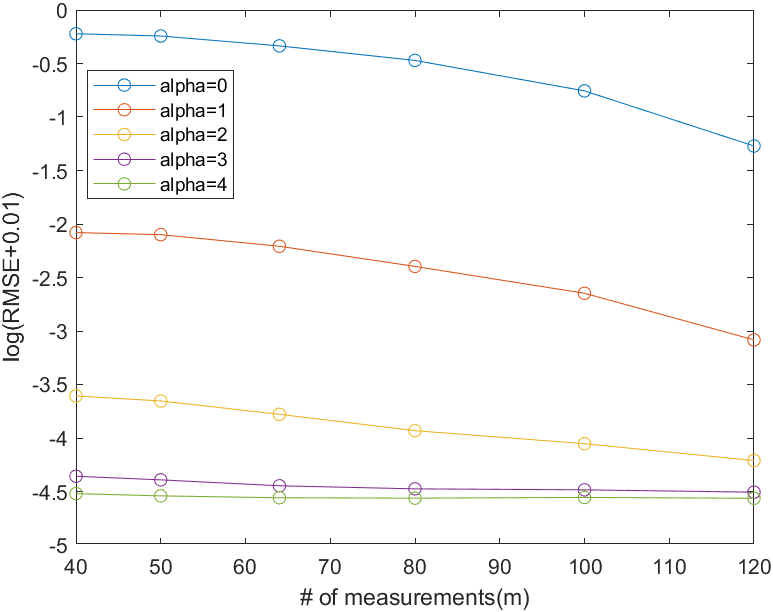
\includegraphics[scale=0.75]{rmse.png}  % change scale factor to re-size the image.
	% give a caption.
	\caption{RMSE vs m}
	% a label to refer to the figure
	\label{fig:1}
\end{figure}
We observe that for the same m, RMSE decreases as $\alpha$ increases. The magnitude of the eigenvalues of the covariance matrix tells us how much the random vector is spread along that direction about the mean. If the eigenvalue along that direction is very small then essentially it means that the random vector is almost constant along that direction. In our case since mean was 0, it means values of $\boldsymbol{x}$ along that direction (or if ith eigenvector is small then ith element) is almost always 0.\\
The structure of the covariance matrix $\Sigma_x$ is that its eigenvalues decreases with increase in the row number which is at faster rate for larger $\alpha$. Due to this most of the values in vector $\boldsymbol{x}$ is zero because of negligibly small eigenvalues. Since most of the values are zero we need lesser number of measurements to estimate the non-zero values in $\boldsymbol{x}$ as $\alpha$ increases.\\
Whereas, for same $\alpha$ RMSE decreases with increase in number of measurements is obvious as more observations would lead to more accurate estimation of $\boldsymbol{x}$.\\
\textbf{Note:} We used a ready made function to generate orthogonal matrix for this question which is uploaded with the file.


\section*{Question 3}
\subsection*{3.a}
$X_0$  is a matrix of rank $r$ such that $\mathcal{A}(X_0) = b$. We also have $X^*$ such that
$$X^* \coloneqq \arg \min \limits_{X} \norm{X}_* \quad \text{subject to } \A(X) = b$$
As $X^*$ is a matrix with minimum nuclear norm subject to the condition $\A(X) = b$ and $X_0$ also satisfies $\A(X_0) = b$, the nuclear norm of $X_0$ should be more than that of $X^*$ i.e.,
$$\norm{X_0}_* \geq \norm{X^*}_*$$
\subsection*{3.b}
$X_0$ and $R_c$ have same dimension by construction. And by theorem (3.3) of the paper, $X_0^\intercal R_c = 0$ and $X_0R_c^\intercal = 0$. Hence, $X_0$ and $R_c$ satisfy the conditions of Lemma (2.3) of the paper and hence
$$\norm{X_0 + R_c}_* = \norm{X_0}_* + \norm{R_c}_*$$
Hence
$$\norm{X_0}_* \geq \norm{X_0 + R}_* \geq \norm{X_0 + R_c}_* - \norm{R_0}_* = \norm{X_0}_* + \norm{R_c}_* - \norm{R_0}_*$$
Using the relationship between the leftmost and the rightmost terms, we get
$$\norm{X_0}_* \geq \norm{X_0}_* + \norm{R_c}_* - \norm{R_0}_*$$
Hence
$$\norm{R_0}_* \geq \norm{R_c}_*$$
\subsection*{3.c}
Without loss of generality, assume that the SVD has been performed in such a way that the singular values are arranged in decreasing order along the diagonal and the corresponding left and right singular vectors are re-ordered. The partitions $I_i$ are disjoint by construction and are $3r$ in cardinality.\\
Consider a singular value $\sigma_k$ of $R_c$ such that $k \in I_{i+1}$. By our assumption above, for every $j \in I_i$, we have
$$\sigma_k \leq \sigma_j$$
Repeating the above inequality for all $j \in I_i$ and then adding those $3r$ inequalities, we get
$$\sigma_k \times 3r \leq \sum \limits_{j \in I_i}\sigma_j$$
hence
$$\sigma_k \leq \frac{1}{3r}\sum \limits_{j \in I_i}\sigma_j$$
\subsection*{3.d}
Note that $\norm{R_i}_* = \sum \limits_{j \in I_i}\sigma_j$. Hence, the above inequality becomes
$$\sigma_k \leq \frac{1}{3r}\norm{R_i}_*$$
Squaring on both sides (as both the sides are positive quantities, the sign of the inequality doesn't change)
$$\sigma_k^2 \leq \frac{1}{9r^2}\norm{R_i}_*^2 \quad \forall k \in I_{i+1}$$
Adding up the above $3r$ inequalities, we get
$$\sum\limits_{k \in I_{i+1}} \sigma_k^2 \leq \frac{3r}{9r^2}\norm{R_i}_*^2$$
But $\norm{R_{i+1}}_F^2 = \sum\limits_{k \in I_{i+1}} \sigma_k^2$. Hence we have
$$\norm{R_{i+1}}_F^2 \leq \frac{1}{3r}\norm{R_i}_*^2$$
\subsection*{3.e}
Using the result derived in 3.d, we have
$$\norm{R_{i+1}}_F \leq \frac{1}{\sqrt{3r}}\norm{R_i}_*$$
Repeating the above inequality and adding all of them, we have
$$\sum \limits_{i \geq 1}\norm{R_{i+1}}_F \leq \frac{1}{\sqrt{3r}}\sum \limits_{i \geq 1}\norm{R_i}_*$$
By change of variable, we have
$$\sum \limits_{j \geq 2}\norm{R_{j}}_F \leq \frac{1}{\sqrt{3r}}\sum \limits_{j \geq 1}\norm{R_j}_*$$
\subsection*{3.f}
As all the $R_j$ have orthogonal row space and column space, by the sub-addivity property of nuclear norm, we have
$$\sum \limits_{j \geq 1}\norm{R_j}_* = \norm{R_c}_*$$
But by equation (3.4) of the paper (which is same as the result in 3.b above), $\norm{R_0}_* \geq \norm{R_c}_*$. Hence
$$\sum \limits_{j \geq 2}\norm{R_{j}}_F \leq \frac{1}{\sqrt{3r}}\sum \limits_{j \geq 1}\norm{R_j}_* = \frac{1}{\sqrt{3r}} \norm{R_c}_* \leq \frac{1}{\sqrt{3r}} \norm{R_0}_*$$
\subsection*{3.g}
As per the construction using the Lemma (3.4) of the paper and as rank of $X_0$ is $r$, we have 
$$\text{rank}(R_0) \leq 2r$$
Since the relation between the nuclear norm and Frobenius norm (from linear algebra) for some matrix $P$ is
$$\norm{P}_* \leq \sqrt{\text{rank}(P)} \, \norm{P}_F$$
applying to $R_0$, we get
$$\norm{R_0}_* \leq \sqrt{2r} \, \norm{R_0}_F$$
Using this in the result of (3.f) above, we finally have
$$\sum \limits_{j \geq 2}\norm{R_{j}}_F \leq \frac{1}{\sqrt{3r}}\sum \limits_{j \geq 1}\norm{R_j}_* = \frac{1}{\sqrt{3r}} \norm{R_c}_* \leq \frac{1}{\sqrt{3r}} \norm{R_0}_* \leq \frac{\sqrt{2r}}{\sqrt{3r}}\norm{R_0}_F$$
\subsection*{3.h}
By construction, $\text{rank}(R_1) \leq 3r$ and by Lemma (3.4) of the paper, $\text{rank}(R_0) \leq 2r$. Hence by subadditivity property of rank, we have
$$\text{rank}(R_0 + R_1) \leq 2r + 3r = 5r$$
\subsection*{3.i}
We have 
$$R = R_0 + R_c = R_0 + R_1 + \sum \limits_{j \geq 2}R_j$$
Hence, by triangle inequality,
$$\norm{\A(R)} = \norm{\A\bigg((R_0 + R_1) + \sum \limits_{j \geq 2}R_j\bigg)} \geq \norm{\A(R_0+R_1)} - \norm{\A\bigg(\sum \limits_{j \geq 2}R_j\bigg)}$$
But again using the triangle inequality, we have
$$\norm{\A\bigg(\sum \limits_{j \geq 2}R_j\bigg)} \leq \sum \limits_{j \geq 2} \norm{\A(R_j)}$$
Hence,
$$\norm{\A(R)} \geq  \norm{\A(R_0+R_1)} - \sum \limits_{j \geq 2} \norm{\A(R_j)}$$
\subsection*{3.j}
As the rank of $R_0 + R_1$ is atmost $5r$ and the rank of $R_j$ is atmost 3r $\forall j \geq 2$, by using the restricted isometry property of $\A$, we have
$$\norm{\A(R_0 + R_1)} \geq (1 - \delta_{5r}) \norm{R_0 + R_1}_F$$
and 
$$\norm{\A(R_j)} \leq (1 + \delta_{3r})\norm{R_j}_F \quad \forall j \geq 2$$
Using the above two inequalities in the result of (3.j) above, we get
\begin{eqnarray*}
	\norm{\A(R)} &\geq&  \norm{\A(R_0+R_1)} - \sum \limits_{j \geq 2} \norm{\A(R_j)}\\
	&\geq& (1 - \delta_{5r}) \norm{R_0 + R_1}_F -  (1 + \delta_{3r})\sum \limits_{j \geq 2} \norm{R_j}_F
\end{eqnarray*}
\subsection*{3.k}
Since $\A$ is an affine transformation and $\A(X^*) = b$ and $\A(X_0) = b$, we have
$$\A(R) = \A(X^* - X_0) = \A(X^*) - \A(X_0) = b - b = 0$$
\subsection*{3.l}
The inequality (3.7) of the paper is as follows:
$$\norm{\A(R)} \geq \bigg((1-\delta_{5r}) - \frac{9}{11}(1+\delta_{3r})\bigg) \norm{R_0}_F$$
Since $\A(R) = 0$, $\norm{\A(R)} = 0$. We know that the Frobenius norm of a matrix is always non-negative. Hence, the right hand side of the above inequality to be positive, we need
$$\bigg((1-\delta_{5r}) - \frac{9}{11}(1+\delta_{3r})\bigg) > 0$$
Taking LCM and then simplifying, we have
$$\frac{2 - (11\delta_{5r} + 9\delta_{3r})}{11} > 0$$
which is equivalent to numerator being positive or
$$11\delta_{5r} + 9\delta_{3r} < 2$$





\section*{Question 4}
Incoherence of singular vectors with the canonical basis is required for matrix recovery to avoid cases where the low rank matrix takes the form such as all zeros except 1 at the any random position or in other words there is not much variation among most of the elements of the matrix except for very few elements where value is significantly different. When random elements of such matrices are sampled most of the time we would observe small variation among the sampled values and we have no way of knowing what were the significantly different values. Matrices of rank less than r can be represented by:
\begin{equation*}
	\boldsymbol{M} = \sum_{i=1}^{r}\sigma_k\boldsymbol{u_k}\boldsymbol{v_k}^T
\end{equation*}
where all the symbols have there usual meanings. When singular vectors are uniformly sampled from the set of all families of r orthonormal vectors we are infact asking for incoherence with the canonical basis so as to avoid pathological cases as described above. This can be seen by taking an example where singular vectors are themselves are standard orthonormal vectors. Each summand in the sum would be a matrix with just one non-zero element making the net matrix have just r$(<min(m,n)$ making the net matrix almost all zeros with r non-zero elements giving us the pathological case we wanted to avoid.\\
When the constraint is changed to:
\begin{equation*}
	minimize \ \ rank(\boldsymbol{X})
\end{equation*}
\begin{equation*}
	subject \ to: \ \ \boldsymbol{f_i}^T\boldsymbol{X}\boldsymbol{g_j} = \boldsymbol{f_i}^T\boldsymbol{M}\boldsymbol{g_j} \ \ (i,j) \in \Omega
\end{equation*}
Using the rank r representation of matrix $\boldsymbol{M}$ we get:
\begin{equation*}
	\boldsymbol{f_i}^T\boldsymbol{M}\boldsymbol{g_j} = \sum_{i=1}^{r}\sigma_k\boldsymbol{f_i}^T\boldsymbol{u_k}\boldsymbol{v_k}^T\boldsymbol{g_j} \ \ (i,j) \in \Omega
\end{equation*}
Again we see, that if the right($\boldsymbol{v_k}$) and left($\boldsymbol{u_k}$) singular vectors are highly coherent with $g_j$ and $f_i$ then again we will get almost all zero matrix with few non-zero elements. Thus, all that is needed is that the column and row spaces of M be respectively incoherent with the basis ($\boldsymbol{f_i}$) and ($\boldsymbol{g_i}$).

\section*{Question 5}
\begin{itemize}
	\item \textbf{Title:} Active Contours with Group Similarity
	\item \textbf{Venue:} Department of ECE, The Hong Kong University of Science and Technology; Image Analysis and Processing Group, Yale University
	\item \textbf{Problem Addressed:} Active contours are widely used in image segmentation. To cope with missing or misleading features in images, researchers have introduced various ways to model the prior of shapes and use the prior to constrain active contours. However, the shape prior is usually learnt from a large set of annotated data, which is not always accessible in practice. Moreover, it is often that the existing shapes in the training set are not sufficient to model the new instance in the testing image. In this paper, the author proposes to use the group similarity of object shapes in multiple images as a prior to aid segmentation. 
	\item \textbf{Method and Objective Function:} The paper proposes to represent each shape contour as a vector. Shape contours of similar objects(may have different size, rotations) are put into a matrix form. Intuitively, this matrix must have small rank because rank gives us an indication of the correlation among the vectors of a matrix. For example, the rank equals to 1 if the shapes are identical, and the rank may increase if some shapes change. Intrinsically, the rank of the shape matrix describes the degree of freedom of the shape change. The low-rank constraint will allow the global change of contours such as translation, scaling, rotation and principal deformation to fit the image data while truncating the local variation caused by image defects. The objective function they seek to minimize is:
	\begin{equation*}
		min_{\boldsymbol{X}}\sum_if_i(C_i) \ \ \textrm{subject to} \ rank(\boldsymbol{X}) \leq K
	\end{equation*}
	where $C_i$ are the contours, $\boldsymbol{X = [\boldsymbol{C_1 \ C_2...C_n}]}$ and $f_i(.)$ is the energy of the active contour. For region-based energy it is given by:
	\begin{equation*}
		f_i(C_i) = \int_{\Omega_1}(I_i(x)-u_1)^2dx+\int_{\Omega_2}(I_i(x)-u_2)^2dx+\beta length(C_i)
	\end{equation*}
	where $I_i(x)$ is the intensity of ith image at pixel location x, $\Omega_1$ and $\Omega_2$ are the regions inside and outside of the contour respectively and $u_1$ and $u_2$ are the mean intensity of pixels inside and outside contour respectively. Since the given objective function is difficult to optimize due to discrete nature a relaxed version of the optimization is given by:
	\begin{equation*}
		min_{\boldsymbol{X}}(\sum_if_i(C_i)+\lambda||\boldsymbol{X}||_*)
	\end{equation*}
	where $||\boldsymbol{X}||_*$ is the nuclear norm of $\boldsymbol{X}$.
\end{itemize}
	
\end{document}
